% !TeX root = ../../../master.tex

\subsection{Ordnerstruktur}
\label{ssec:Ordnerstruktur}

Wie bereits in den Kapiteln \myRefGeneral{ssec:React} und \myRefGeneral{ssec:AufbauReact} dargelegt, werden für den Aufbau der Anwendung verschiedene Komponenten benötigt. 

Abb. \myRefGeneral{fig:OrdnerstrukturVSCode} zeigt einen Ausschnitt der Ordnerstruktur in der Entwicklungsumgebung \emph{Visual Studio Code (VS Code)}.\footnote{\url{https://code.visualstudio.com}}
Exemplarisch werden kurz die Card-Komponente sowie die Admin-Komponente erläutert, deren Ergebnisse später in Kapiteln A, B, aufgezeigt werden. \todo[]{Ref Chapter}

Für jede Komponente wird in VS Code ein eigener Ordner angelegt, der die Komponente selbst (wie z.B. \jinline|Admin| oder \jinline|Card|) sowie die Kind-Komponenten (wie z.B. \jinline|CreateUserCard|) enthält.  
Des weitern wird eine spezifische \emph{\acs{CSS}}-Datei angelgt, die Anpassungen an den \acsu*{HTML}-Dateien vollzieht. 
Dies könnte z.B. die Farbe in \enquote{DHBW-rot} sein. 
Damit einhergehend kann eine differenzierterer und übersichtlicher Code erzeugt werden. 

Wie bereits beschrieben kann eine Komponente mehrere Kind-Komponenten und diese ebenfalls wieder mehrere Kind-Komponenten enthalten. 
So fungiert die Klasse \jinline|Card| u.a. als Kind-Komponente der Komponente \jinline|CreateUserCard|, \jinline|RegisterKeyCard| und \jinline|ShowUsersCard|. 

\begin{figure}[!h]
	\centering
	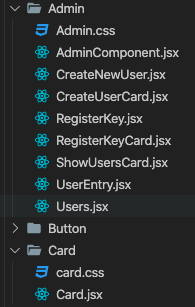
\includegraphics[height=0.4\textwidth, keepaspectratio]{img/client/ordnerStruktur.png}
	\captionsetup{justification=centering, format=plain}
	\caption[Ordnerstruktur in Visual Studio Code]{Ordnerstruktur in Visual Studio Code \\ \quelleScreenshot}
	\label{fig:OrdnerstrukturVSCode}
\end{figure}
